\section{Esercizio 9}
\textit{\textbf{Descrizione:} Scrivere una function Matlab che, data in ingresso la matrice \textbf{LU} ed il vettore \textbf{p} creati dalla function del precedente esercizio, ed il termine noto del sistema lineare \textbf{Ax = b}, ne calcoli la soluzione: \textbf{function x = lusolve(LU,p,b)}. Curare particolarmente la scrittura e l'efficienza della function.}\newline

\noindent \textit{\textbf{Svolgimento:}}\newline

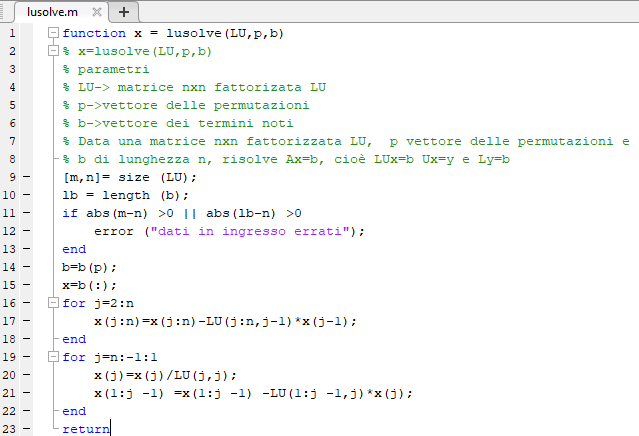
\includegraphics[width=1.3\linewidth]{img/lusolve.png}\newpage